\documentclass[11pt, oneside]{article}   	% use "amsart" instead of "article" for AMSLaTeX format
\usepackage{geometry}                		% See geometry.pdf to learn the layout options. There are lots.
\geometry{letterpaper}                   		% ... or a4paper or a5paper or ... 
%\geometry{landscape}                		% Activate for for rotated page geometry
%\usepackage[parfill]{parskip}    		% Activate to begin paragraphs with an empty line rather than an indent
\usepackage{graphicx}				% Use pdf, png, jpg, or eps� with pdflatex; use eps in DVI mode
								% TeX will automatically convert eps --> pdf in pdflatex		
\usepackage{amssymb}
\usepackage{amsmath}
\usepackage{parskip}
\usepackage{color}
\usepackage{hyperref}

\title{Integrating functions of a complex variable}
%\author{The Author}
%\section{}
%\subsection*{}
\date{}							% Activate to display a given date or no date

\graphicspath{{/Users/telliott_admin/Dropbox/Tex/png/}}
% \begin{center} 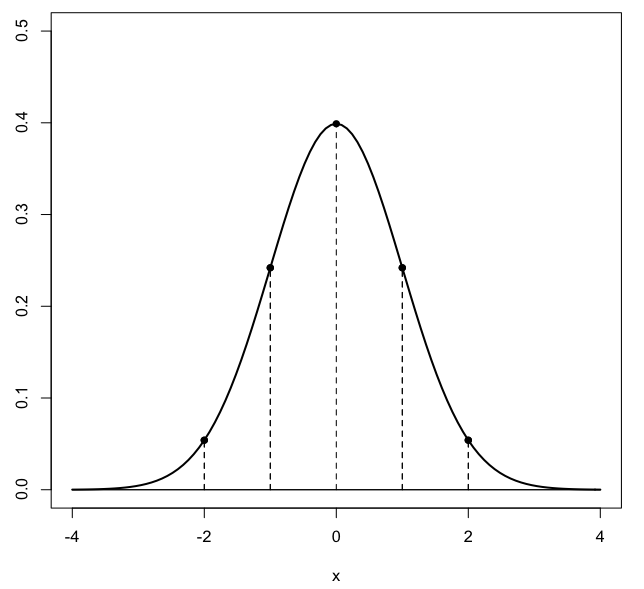
\includegraphics [scale=0.4] {gauss3.png} \end{center}
\begin{document}
\maketitle
\Large
Complex functions are differentiated and integrated in a way that is similar to real functions, with these differences:  

\begin{itemize}
  \item we typically restrict attention to analytic functions 
  \item the integrals that we compute are line integrals along some path
  \item we pay attention to points in the complex plane with poles (or singularities)
\end{itemize}

In general terms, if we have
\[ z = x + i y \]
\[ dz = dx + i dy \]
and the function
\[ w = f(z) = u(x,y) + iv(x,y) \]
we can write
 \[ \int f(z) \ dz = \int (u + i v) (dx + i dy) \]
\[ = \int u \ dx - \int v \ dy + i \ [ \ \int v \ dx + \int u \ dy \ ] \]
What was an integral of a complex function has been transformed into two integrals of real variables, where the real variables are related by the curve over which we will integrate.  

Just as with line integrals for real functions of $x$ and $y$, this is \emph{not} some kind of double integral in both variables.  We can view $y$ as a function of $x$ or perhaps, we can parametrize both $x$ and $y$ as functions of $t$.

Recall that for the work integral
\[ \int_C \mathbf{F} \cdot d \mathbf{r} = M \ dx + N \ dy \]
we parametrize the curve to get the integral over a single variable.

Suppose our function is simply $z = x + iy$.  The integral is 
\[ \int z \ dz = \int (x + iy) (dx + i dy) \]
\[ = \int x \ dx - y \ dy + i x \ dy + i y \ dx \]
We use the curve to get $y=f(x)$ or both $x$ and $y$ as functions of some parameter $t$.

\end{document}  